\documentclass[12pt,twoside]{article}
\usepackage{jmlda}
%\NOREVIEWERNOTES
\title
    %[Образец оформления статьи для публикации] % Краткое название; не нужно, если полное название влезает в~колонтитул
    {Оценка энергии связывания белка и маленьких молекул}
\author
    %[Грачева~А.\,С.] % список авторов для колонтитула; не нужен, если основной список влезает в колонтитул
    {Анастасия Грачева, Мария Кадукова, Сергей Грудинин, В.В. Стрижов} % основной список авторов, выводимый в оглавление
    %[Автор~И.\,О.$^1$, Соавтор~И.\,О.$^2$, Фамилия~И.\,О.$^2$] % список авторов, выводимый в заголовок; не нужен, если он не отличается от основного

\email
    {gracheva.as@phystech.edu}

\abstract
    {При разработке лекарства возникает задача поиска маленьких молекул -- лигандов, наиболее сильно взаимодействующих с исследуемым белком, а значит являющихся основными кандидатами в лекарства. Один из способов определить действительное положение такого лиганда заключается в том, чтобы генерировать несколько возможных положений и классифицировать их как нативные, то есть реально встречающиеся и не нативные. Но качество предсказания может быть повышено, если использовать экспериментальные данные о свободной энергии связывания молекул и решать одновременно задачи регрессии и классификации. В статье будут рассмотрены эксперименты с алгоритмом, использующим эту идею.
    

%\bigskip
\textbf{Ключевые слова}: \emph {машинное обучение, SVM, выпуклая оптимизация, молекулярный докинг, белково-лигандные взаимодействия}.
}
\titleEng
    {JMLDA paper example: file jmlda-example.tex}
\authorEng
    {Author~F.\,S.$^1$, CoAuthor~F.\,S.$^2$, Name~F.\,S.$^2$}
\organizationEng
    {$^1$Organization; $^2$Organization}
\abstractEng
    {This document is an example of paper prepared with \LaTeXe\
    typesetting system and style file \texttt{jmlda.sty}.

    \bigskip
    %\textbf{Keywords}: \emph{keyword, keyword, more keywords}.
}
\begin{document}
\maketitle
%\linenumbers
\section{Введение}
Предсказание наиболее выгодной ориентации и положения молекул по отношению друг к другу для образования устойчивого \emph{комплекса} из белка и лиганда, или молекулярный докинг\cite{docking} -- задача, важная для ускорения процесса разработки новых лекарств.
Есть два метода её решения: \emph{pose prediction} -- среди нескольких сгенерированных положений лиганда в белке определить наиболее близкое к нативному и \emph{scoring} -- предсказать аффинность (свободную энергию связывания) для комплексов различных белков с лигандами. При этом положение с наименьшей энергией связывания будет соответствовать нативной конформации. Первая задача решена в работе с помощью оптимизации скоринговой функции, учитывающей всевозможные комбинации различных пар атомов и расстояния между ними. Раскладывая эту функцию по базису, авторы представляют её как вектор структурных коэффициентов и сводят задачу к модифицированной SVM-классификации.

Наше предположение заключается в том, что с использованием экспериментальных данных об аффинностях можно улучшить качество классификации. В эксперименте, описанном в данной статье, мы проверим эту гипотезу, а также постараемся решать оптимизационную задачу максимально эффективно вычислительно, чтобы использовать как можно больше доступных экспериментальных  данных.

\section{Модель взаимодействий}

Пусть имеется $P$ нативных комплексов белков-лигандов $\{C_{i0}\}_{i=1}^P$. Применив к лигандам изометрические преобразования, сгенерируем для каждой нативной позы $D$ ненативных поз $\{C_{ij}\}_{j=1}^D$. Таким образом, для каждого из $P$ комплексов имеем $(D + 1)$ конформаций: одну нативную и $D$ ненативных. Требуется найти скоринговый функционал $E$, который удовлетворяет следующим неравенствам: 
\begin{equation}\label{eq1}
E(C_{i0}) < E(C_{ij}) \ \forall i\in\{1,\dots,P\}, \ \forall j\in\{1,\dots,D\}.
\end{equation}

В качестве такого функционала будем рассмаривать свободную энергию связывания белков с лигандами, определенную для всех возможных комплексов. Для упрощения формы функционала сделаем ряд допущений.

Во-первых, будем рассматривать комплекс "белок-лиганд"\ как набор атомов, каждый из которых имеет некоторый тип. Тип каждого атома зависит от его химических свойств, таких как номер элемента в периодической таблице, аромат, гибридизация, полярность и т.д. Пусть $M_1$ -- количество типов атомов лиганда, а $M_2$ -- количество типов атомов белка. Тогда получим всего $M_1\times M_2$ различых атомных взаимодействий.

Во-вторых, будем считать, что $E$ определяется только взаимодействиями между парами атомов рассматриваемого комплекса. При этом в каждой паре первый атом является атомом лигнда, а второй -- атомом белка. Кроме того, будем рассматривать только те пары, в которых расстояние между атомами не превышает некоторой пороговой величины $r_{\max}$. В качестве $r_{\max}$ возьмем значение $10$\AA, как это было сделано в других работах \cite{rmax1,rmax2,rmax3,rmax4,rmax5,rmax6} ранее. 

В-третьих, будем считать, что $E$ зависит только от распределения расстояний между взаимодействующими атомами. 

И, наконец, предположим, что $E$ является линейным функционалом и имеет вид: 
\begin{equation}\label{eq2}
E(n(r)) = \sum_{k=1}^{M_1}\sum_{l=1}^{M_2}\int_{0}^{r_{max}}n^{kl}(r)f^{kl}(r)dr,
\end{equation}
где $f^{kl}(r)$ -- неизвестные функции взаимодествия между атомами типов $k$ и $l$. Будем называть их \textit{скоринговыми потенциалами}. Функции $n^{kl}(r)$ -- численные плотности распределений пар атомов типов $k$ и $l$ по расстоянию $r$ между ними: 
\begin{equation}\label{eq3}
n^{kl}(r) = \sum_{i,j} \frac{1}{\sqrt{2\pi\sigma^2}} \exp\left[{-\frac{(r-r_{ij})^2}{2\sigma^2}}\right],
\end{equation}
где $\sigma^2$ -- стандартное отклонение (константа). Сумма берется по всем парам $(i, j)$ атомов с типами $k$ и $l$ соответственно, у которых расстояние между атомами не превышает пороговой величины $r_{\max}$, атом $i$ принадлежит лиганду, а атом $j$ -- белку.

Разложим неизвестные скоринговые потенциалы $f^{kl}(r)$ и плотности $n^{kl}(r)$ по полиномиальному базису: 
\begin{equation}\label{eq4}
\begin{split}
f^{kl}(r) & = \sum_{q} w_q^{kl}\psi_q(r), \\
n^{kl}(r) & = \sum_{q} x_q^{kl}\psi_q(r),
\end{split}
\end{equation}
где $\psi_q(r)$ -- ортогональные базисные функции на интервале $[0, r_{\max}]$, а $w_q^{kl}$ и $x_q^{kl}$ -- коэффициенты разложения функций $f^{kl}(r)$ и $n^{kl}(r)$ соответственно. Поскольку базисные функции ортогональны, справедливо следующее соотношение:

\begin{equation}\label{eq5}
\int_{0}^{r_{\text{max}}}\psi_i(r)\psi_j(r)\Omega(r)dr = \delta_{ij}, \ r\in[0,r_{\text{max}}],
\end{equation}
где $\Omega(r)$ -- некоторая неотрицательная весовая функция на $[0,r_{\text{max}}]$, $\delta_{ij}$ -- символ Кронекера. Из данного условия \eqref{eq5} ортогональности базисных функций могут быть найдены коэффициенты раложения $w_q^{kl}$ и $x_q^{kl}$:
\begin{equation}\label{eq6}
\begin{split}
w_q^{kl}=\int_{0}^{r_{\text{max}}}f_{kl}(r)\psi_q(r)dr, \\
x_q^{kl}=\int_{0}^{r_{\text{max}}}n_{kl}(r)\psi_q(r)dr,
\end{split}
\end{equation}

Таким образом, функционал $E$ можно записать в следующем виде:
\begin{equation}\label{eq7}
E(n(r)) = \sum_{k=1}^{M_1} \sum_{l=1}^{M_2} \sum_{pq}^{\infty}w_q^{kl}x_p^{kl}\int_{0}^{r_{\text{max}}}\psi_q(r)\psi_p(r)\Omega(r)dr.
\end{equation}

Учитывая условие ортогональности \eqref{eq5} и ограничиваясь порядком разложения Q, получаем приближенное выражение скорингового функционала: 
\begin{equation}\label{eq8}
\begin{split}
E(n(r)) \approx \sum_{k=1}^{M_1} & \sum_{l=1}^{M_2} \sum_{q=0}^{Q}w_q^{kl}x_q^{kl} = \langle\mathbf{w},\mathbf{x}\rangle,\\
\mathbf{w}, \mathbf{x} & \in \mathbb{R}^{Q\times M_1\times M_2}.
\end{split}
\end{equation}

Неизвестный вектор $\mathbf{w}$ будем называть \textit{скоринговым вектором}, а вектор $\mathbf{x}$ -- \textit{структурным вектором}. Структурный вектор известен для решения задачи: его можно получить из данных. Для оценки энергии связывания в работе \cite{regression} использовался порядок разложения $Q=10$, и рассматривались $M_1 = 48$ типов атомов.

\section{Постановка задачи}
Пусть $\{C_{ij}\}_{i=1}^P$ -- комплексы белков и лигандов. При $j=0$ они находятся в нативных позах, при $j = 1 \dots D$ -- в ненативных. Задача заключается в том, чтобы найти скоринговую функцию $E$, который удовлетворяет неравенствам: 
\begin{equation}\\
\begin{split}
& E(C_{i0}) < E(C_{ij}) \\
& \forall i\in 1,\dots,P, \\
& \forall j\in 1,\dots,D.
\end{split}
\end{equation}

В модели взаимодействия, описанной в [1], эта функция задаётся скоринговым вектором $\mathbf{w}$. Поэтому неравенство выше может быть преобразовано в систему неравенств:
 
\begin{equation}\label{eq9}
\begin{split}
& \langle\mathbf{x}_{i0}, \mathbf{w}\rangle < \langle\mathbf{x}_{ij}, \mathbf{w}\rangle, \\
& \langle\mathbf{x}_{ij} - \mathbf{x}_{i0}, \mathbf{w}\rangle > 0, \\
& \forall i = 1,\dots, P, \\
& \forall j = 1, \dots, D.
\end{split}
\end{equation}
где $x_{ij}$ -- структурные вектора.  

Чтобы гарантировать единственность решения, а также решать задачу в случае линейной неразделимости выборки, приведём её к виду задачи квадратичной оптимизации с мягким зазором:
\begin{equation}\label{eq10}
\begin{aligned}
& \underset{\mathbf{w}, b_i, \xi_{ij}}{\text{minimize:}}
& & \frac{1}{2} \|\mathbf{w}\|^2 + C\sum\limits_{ij}\xi_{ij} \\
& \text{subject to:}
& & y_{ij}[\langle\mathbf{w},\mathbf{x}_{ij}\rangle - b_i]-1+\xi_{ij} \geq 0, \\
&&& \xi_{ij} \geq 0,\\
&&&i\in\{1,\dots,P\}, \\
&&&j\in\{0,\dots,D\},
\end{aligned}
\end{equation}
где $\mathbf{w}$, $b_i$ и переменные невязки $\xi_{ij}$ -- оптимизируемые параметры модели, \\
$y_{i0}=1$ для нативной позы и $y_{ij}=-1, \ j\in\{1,\dots,D\},$ для ненативной,\\
а $C$ -- некоторый коэффициент регуляризации. \\
Таким образом, решив оптимизационную задачу, решаем и задачу класификации.

Кроме того, есть другая постановка этой задачи -- задача регрессии, т.е. предсказания значения свободной энергии связывания белка с лигандом:
\begin{equation}\label{eq11}
\begin{aligned}
& \underset{\mathbf{w}}{\text{minimize:}}
& & \sum\limits_{i}[\langle\mathbf{w},\mathbf{x}_{i0}\rangle - s_i]^2 + \alpha\|\mathbf{w}\|^2, \\
&&& i\in\{1,\dots,P\},
\end{aligned}
\end{equation}
где $s_i$ -- экспериментально полученное значение энергии связывания $i$-го нативного соединения, $\alpha$ -- коэффициент регуляризации для ridge-регрессии. 

Объединение этих методов заключается в сложении функций потерь классификации и регрессии:
\begin{equation}\label{eq12}
\begin{aligned}
& \underset{\mathbf{w}, b_i, \xi_{ij}}{\text{minimize:}}
& & \frac{1}{2} \|\mathbf{w}\|^2 + C\sum\limits_{ij}\xi_{ij} + C_{r}\sum\limits_{i} f(\mathbf{x}_{i0},\mathbf{w}, s_i) \\
& \text{subject to:}
& & y_{ij}[\langle\mathbf{w},\mathbf{x}_{ij}\rangle - b_i]-1+\xi_{ij} \geq 0, \\
&&& \xi_{ij} \geq 0, \\
&&&i\in\{1,\dots,P\}, \\
&&&j\in\{0,\dots,D\},
\end{aligned}
\end{equation}
где $f(\mathbf{x}_{i0},\mathbf{w}, s_i)$ -- MSE, $C_r$ -- коэффициент регуляризации для функции потерь регрессии. 

\section{Теоретическая часть}
С помощью замены переменных сведем два квадратичных слагаемых в целевой функции из задачи \eqref{eq12} к одному. 

Функция потерь регрессии MSE для одного комплекса выражается формулой:
\begin{equation}\label{eq15}
f({\mathbf{x}}_{i0}, {\mathbf{w}}, s_i) = (\langle{\mathbf{x}}_{i0}, {\mathbf{w}} \rangle - s_i)^2.
\end{equation}

Тогда для выборки ${\mathbf{X}}=({\mathbf{x}}_{10}, \dots, {\mathbf{x}}_{P0})^{\text{T}}$, состоящей из нативных конфигураций, и целевого вектора  $\mathbf{s}=(s_1,\dots,s_P)^{\text{T}}$ квадратичные слагаемые целевой функции из задачи \eqref{eq12} принимают вид:
\begin{equation*}
\begin{aligned}
& \frac{1}{2} \|{\mathbf{w}}\|^2 + C_{r}\sum\limits_{i} f({\mathbf{x}}_{i0},{\mathbf{w}}, s_i)=\frac{1}{2}{\mathbf{w}}^{\text{T}}{\mathbf{w}}+C_{r}\|{\mathbf{X}}{\mathbf{w}} - \mathbf{s}\|^2 =\\
& = \frac{1}{2}{\mathbf{w}}^{\text{T}}{\mathbf{w}}+ C_{r}{\mathbf{w}}^{\text{T}}{\mathbf{X}}^{\text{T}}{\mathbf{X}}{\mathbf{w}}- 2C_{r}{\mathbf{w}}^{\text{T}}{\mathbf{X}}^{\text{T}}\mathbf{s} + C_{r}\mathbf{s}^{\text{T}}\mathbf{s}=\\
& = \frac{1}{2}{\mathbf{w}}^{\text{T}}\left(\mathbf{I} + 2C_{r}{\mathbf{X}}^{\text{T}}{\mathbf{X}}\right){\mathbf{w}}- 2C_{r}{\mathbf{w}}^{\text{T}}{\mathbf{X}}^{\text{T}}\mathbf{s}+ C_{r}\mathbf{s}^{\text{T}}\mathbf{s}=\\
& = \frac{1}{2}\left\|\left[\mathbf{I} + 2C_{r}{\mathbf{X}}^{\text{T}}{\mathbf{X}}\right]^{\frac{1}{2}}{\mathbf{w}}\right\|^2- 2C_{r}\left({\mathbf{w}}^{\text{T}}\left[\mathbf{I} + 2C_{r}{\mathbf{X}}^{\text{T}}{\mathbf{X}}\right]^{\frac{1}{2}}\right)
\left(\left[\mathbf{I} + 2C_{r}{\mathbf{X}}^{\text{T}}{\mathbf{X}}\right]^{-\frac{1}{2}}
{\mathbf{X}}^{\text{T}}\mathbf{s}\right)+ C_{r}\mathbf{s}^{\text{T}}\mathbf{s}=\\
& = \left(\left[\mathbf{I} + 2C_{r}{\mathbf{X}}^{\text{T}}{\mathbf{X}}\right]^{\frac{1}{2}}{\mathbf{w}} - C_r\left[\mathbf{I} + 2C_{r}{\mathbf{X}}^{\text{T}}{\mathbf{X}}\right]^{-\frac{1}{2}}
{\mathbf{X}}^{\text{T}}\mathbf{s}\right)^2 + C_r\mathbf{s}^{\text{T}}\mathbf{s}- C_r^2\left\|\left[\mathbf{I} + 2C_{r}{\mathbf{X}}^{\text{T}}{\mathbf{X}}\right]^{-\frac12}
{\mathbf{X}}^{\text{T}}\mathbf{s}\right\|^2.
\end{aligned}
\end{equation*}
Введем замену переменных:
\begin{equation}\label{eq16}
\begin{aligned}
& \mathbf{w}'= \mathbf{A}{\mathbf{w}} - \mathbf{B}, \ \text{где} \\
& \mathbf{A}=\left[\mathbf{I} + 2C_{r}{\mathbf{X}}^{\text{T}}{\mathbf{X}}\right]^{\frac{1}{2}},\\
& \mathbf{B}=C_r\left[\frac{1}{2}\mathbf{I} + C_{r}{\mathbf{X}}^{\text{T}}{\mathbf{X}}\right]^{-\frac{1}{2}}
{\mathbf{X}}^{\text{T}}\mathbf{s}.
\end{aligned}
\end{equation}
Тогда, учитывая, что 
\begin{equation*}
C_r\mathbf{s}^{\text{T}}\mathbf{s}-
C_r^2\left\|\left[\frac{1}{2}\mathbf{I} + C_{r}{\mathbf{X}}^{\text{T}}{\mathbf{X}}\right]^{-\frac12}
{\mathbf{X}}^{\text{T}}\mathbf{s}\right\|^2
=\text{const},
\end{equation*}
задача оптимизации принимает вид: 
\begin{equation}\label{eq17}
\begin{aligned}
& \underset{\mathbf{w}', b_i, \xi_{ij}}{\text{minimize:}}
& & \frac{1}{2} \|\mathbf{w}'\|^2 + C\sum\limits_{ij}\xi_{ij} \\
& \text{subject to:}
& & y_{ij}[\left(\mathbf{A}^{-1}\left(\mathbf{w}'+\mathbf{B}\right)\right)^{\text{T}}\mathbf{x}_{ij} - b_i]-1+\xi_{ij} \geq 0, \\
&&& \xi_{ij} \geq 0, \\
&&&i\in\{1,\dots,P\}, \\
&&&j\in\{0,\dots,D\}.
\end{aligned}
\end{equation}
Введем обозначение:
\begin{equation}\label{eq18}
\hat{\mathbf{X}} = (\mathbf{A}^{-1})^{\text{T}}\mathbf{X}.
\end{equation}

Найдём двойственную задачу:
\begin{equation}
\begin{aligned}
& \mathcal{L}(\mathbf{w}', \mathbf{b}, \mathbf{\xi}, \lambda, r) = \frac{1}{2} \|\mathbf{w}'\|^2 + C\sum\limits_{ij}\xi_{ij} - 
\sum_{ij}{\lambda_{ij} \left( y_{ij}[\langle \mathbf{A}^{-1}\left(\mathbf{w}'+\mathbf{B}\right), \mathbf{x}_{ij}\rangle - b_i]-1+\xi_{ij} \right)} -
\sum_{ij}{r_{ij}\xi_{ij}} \\
& \frac{\partial{\mathcal{L}}}{\partial{\mathbf{w}'}} = \mathbf{w}' - \sum{\lambda_{ij}y_{ij}\langle \mathbf{A}^{-1}\left(\mathbf{w}'+\mathbf{B}\right), \mathbf{x}_{ij} \rangle}'_{w'} = 0 \rightarrow \mathbf{w}' = \sum_{ij}{\lambda_{ij}y_{ij}\mathbf{A}^{-1} \mathbf{x}_{ij}} \\
& \forall i, 
\frac{\partial{\mathcal{L}}}{\partial{b_i}} = \sum_j{\lambda_{ij}y_{ij}} = 0 \\
& \forall (i, j), \frac{\partial{\mathcal{L}}}{\partial{\xi_{ij}}} = C - \lambda_{ij} - r_{ij} = 0 \rightarrow \lambda_{ij} + r_{ij} = C
\end{aligned}
\end{equation}
\begin{equation}
\begin{aligned}
& \mathcal{L}(\lambda, r) = \frac{1}{2} \langle \sum_{ij}{\lambda_{ij}y_{ij}\mathbf{A}^{-1} \mathbf{x}_{ij}}, \sum_{ij}{\lambda_{ij}y_{ij}\mathbf{A}^{-1} \mathbf{x}_{ij}} \rangle + C\sum\limits_{ij}\xi_{ij} - 
\sum_{ij}{\lambda_{ij} y_{ij}\langle \mathbf{A}^{-1} \sum_{ij}{\lambda_{ij}y_{ij} \mathbf{A}^{-1}  \mathbf{x}_{ij}}, \mathbf{x}_{ij}\rangle} - \\ 
& - \sum_{ij}{\lambda_{ij} y_{ij}\langle \mathbf{A}^{-1}\mathbf{B}, \mathbf{x}_{ij} \rangle} + \sum_{ij}{\lambda_{ij} y_{ij}b_i} + \sum_{ij}{\lambda_{ij}}  - \sum_{ij}{\lambda_{ij}\xi_{ij}}- \sum_{ij}{r_{ij}\xi_{ij}} = \\
& = \frac{1}{2} \sum_{ij}\sum_{pq} {\lambda_{ij}\lambda_{pq}y_{ij}y_{pq}\langle \mathbf{A}^{-1} \mathbf{x}_{ij}, \mathbf{A}^{-1} \mathbf{x}_{pq} \rangle} + \sum_{ij}{\xi_{ij}(C - \lambda_{ij} - r_{ij})} - \sum_{ij}\sum_{pq} {\lambda_{ij}\lambda_{pq}y_{ij}y_{pq}\langle \mathbf{A}^{-2} \mathbf{x}_{ij},  \mathbf{x}_{pq} \rangle} - \\
& - \sum_{ij}{\lambda_{ij} y_{ij}\langle \mathbf{A}^{-1}\mathbf{B}, \mathbf{x}_{ij} \rangle} + \sum_{i}{b_i \sum_j{\lambda_{ij} y_{ij}}} + \sum_{ij}{\lambda_{ij}}
\end{aligned}
\end{equation}
\\
\begin{enumerate}
	\item $\sum_{ij}{\xi_{ij}(C - \lambda_{ij} - r_{ij})} = 0$ из ограничений;
	\item $\sum_{i}{b_i \sum_j{\lambda_{ij} y_{ij}}} = 0$ из ограничений;
	\item $\langle  \mathbf{A}^{-2} \mathbf{x},  \mathbf{x} \rangle = \langle  \mathbf{A}^{-1} \mathbf{x}, \mathbf{A}^{-1} \mathbf{x} \rangle$, т.к. $\mathbf{x}^{\top}\mathbf{A}^{-2} \mathbf{x} =  \mathbf{x}^{\top}\mathbf{A}^{-1}\mathbf{A}^{-1} \mathbf{x} = (\mathbf{A}^{-1} \mathbf{x})^{\top}\mathbf{A}^{-1} \mathbf{x}$
\end{enumerate}

$\rightarrow$ введём обозначение:
$\widehat{\mathbf{X}} = (\mathbf{A}^{-1})^{\text{T}}\mathbf{X} = \mathbf{A}^{-1}\mathbf{X}$, т.к. $ \mathbf{A}$ симметрична.
\begin{equation}
\begin{aligned}
& \mathcal{L}(\lambda) = - \frac{1}{2} \sum_{ij}\sum_{pq} {\lambda_{ij}\lambda_{pq}y_{ij}y_{pq}\langle \widehat{\mathbf{x}_{ij}}, \widehat{\mathbf{x}_{pq}} \rangle} - 
\sum_{ij}{\lambda_{ij}y_{ij}\langle \mathbf{A}^{-1}\mathbf{B}, \mathbf{x}_{ij} \rangle} + \sum_{ij}{\lambda_{ij}} = \\
& = - \frac{1}{2} \sum_{ij}\sum_{pq} {\lambda_{ij}\lambda_{pq}y_{ij}y_{pq}\langle \widehat{\mathbf{x}_{ij}}, \widehat{\mathbf{x}_{pq}}  \rangle} + 
\sum_{ij}{\lambda_{ij} \left(1  - y_{ij}\langle \mathbf{B}, \widehat{\mathbf{x}_{ij}} \rangle \right)}
\end{aligned}
\end{equation}
Двойственная задача: $\argmax_{\lambda} \mathcal{L}(\lambda)$

Значит, исходная задача по теореме Каруша-Куна-Таккера эквивалентна двойственной:
\begin{equation}\label{eq19}
\begin{aligned}
& \underset{\lambda_{ij}}{\text{minimize:}}
& & \frac{1}{2}\sum\limits_{(i,j),(p,q)}\lambda_{ij}\lambda_{pq}y_{ij}y_{pq}\langle \widehat{\mathbf{x}}_{ij},\widehat{\mathbf{x}}_{pq}\rangle + \sum_{ij}{\lambda_{ij} \left(y_{ij}\langle \mathbf{B}, \widehat{\mathbf{x}_{ij}} \rangle - 1 \right)} \\
& \text{subject to:}
& & 0\leq\lambda_{ij} \leq C, \\
&&& \forall i, \sum_j{\lambda_{ij}y_{ij}} = 0 \\
&&&i\in\{1,\dots,P\}, \\
&&&j\in\{0,\dots,D\}.
\end{aligned}
\end{equation}

\section{Эксперимент}

Так как множество сильно зависимых между собой примеров, которые могли в том числе встретиться в обучающей и тестовой выборке, не позволяли адекватно оценить качество классификации, было принято решение рассмотреть матрицу корреляции всей имеющейся выборки X и разбить строки из неё на 2 подмножества, не имеющих между собой коэффициентов корреляции $> 0.5$. Получилась тестовая выборка размера около 8\% от всего набора данных.
Кроме того, из-за memory issue в квадратичном солвере обучение удалось провести только на 800 белково-лигандных комплексах (по 19 поз в каждом).

На графиках можно увидеть метрики классификации нативных поз и MSE относительно реальных значений энергии связывания. Так как данные получены до поправки, описанной в начале раздела, и классификатор обучен на небольшом количестве данных, то их нельзя считать окончательными и проводить сравнение с другими исследованиями, так как скорее всего модель переобучилась. 

\begin{figure}[H]
	\subfloat[Точность классификации]{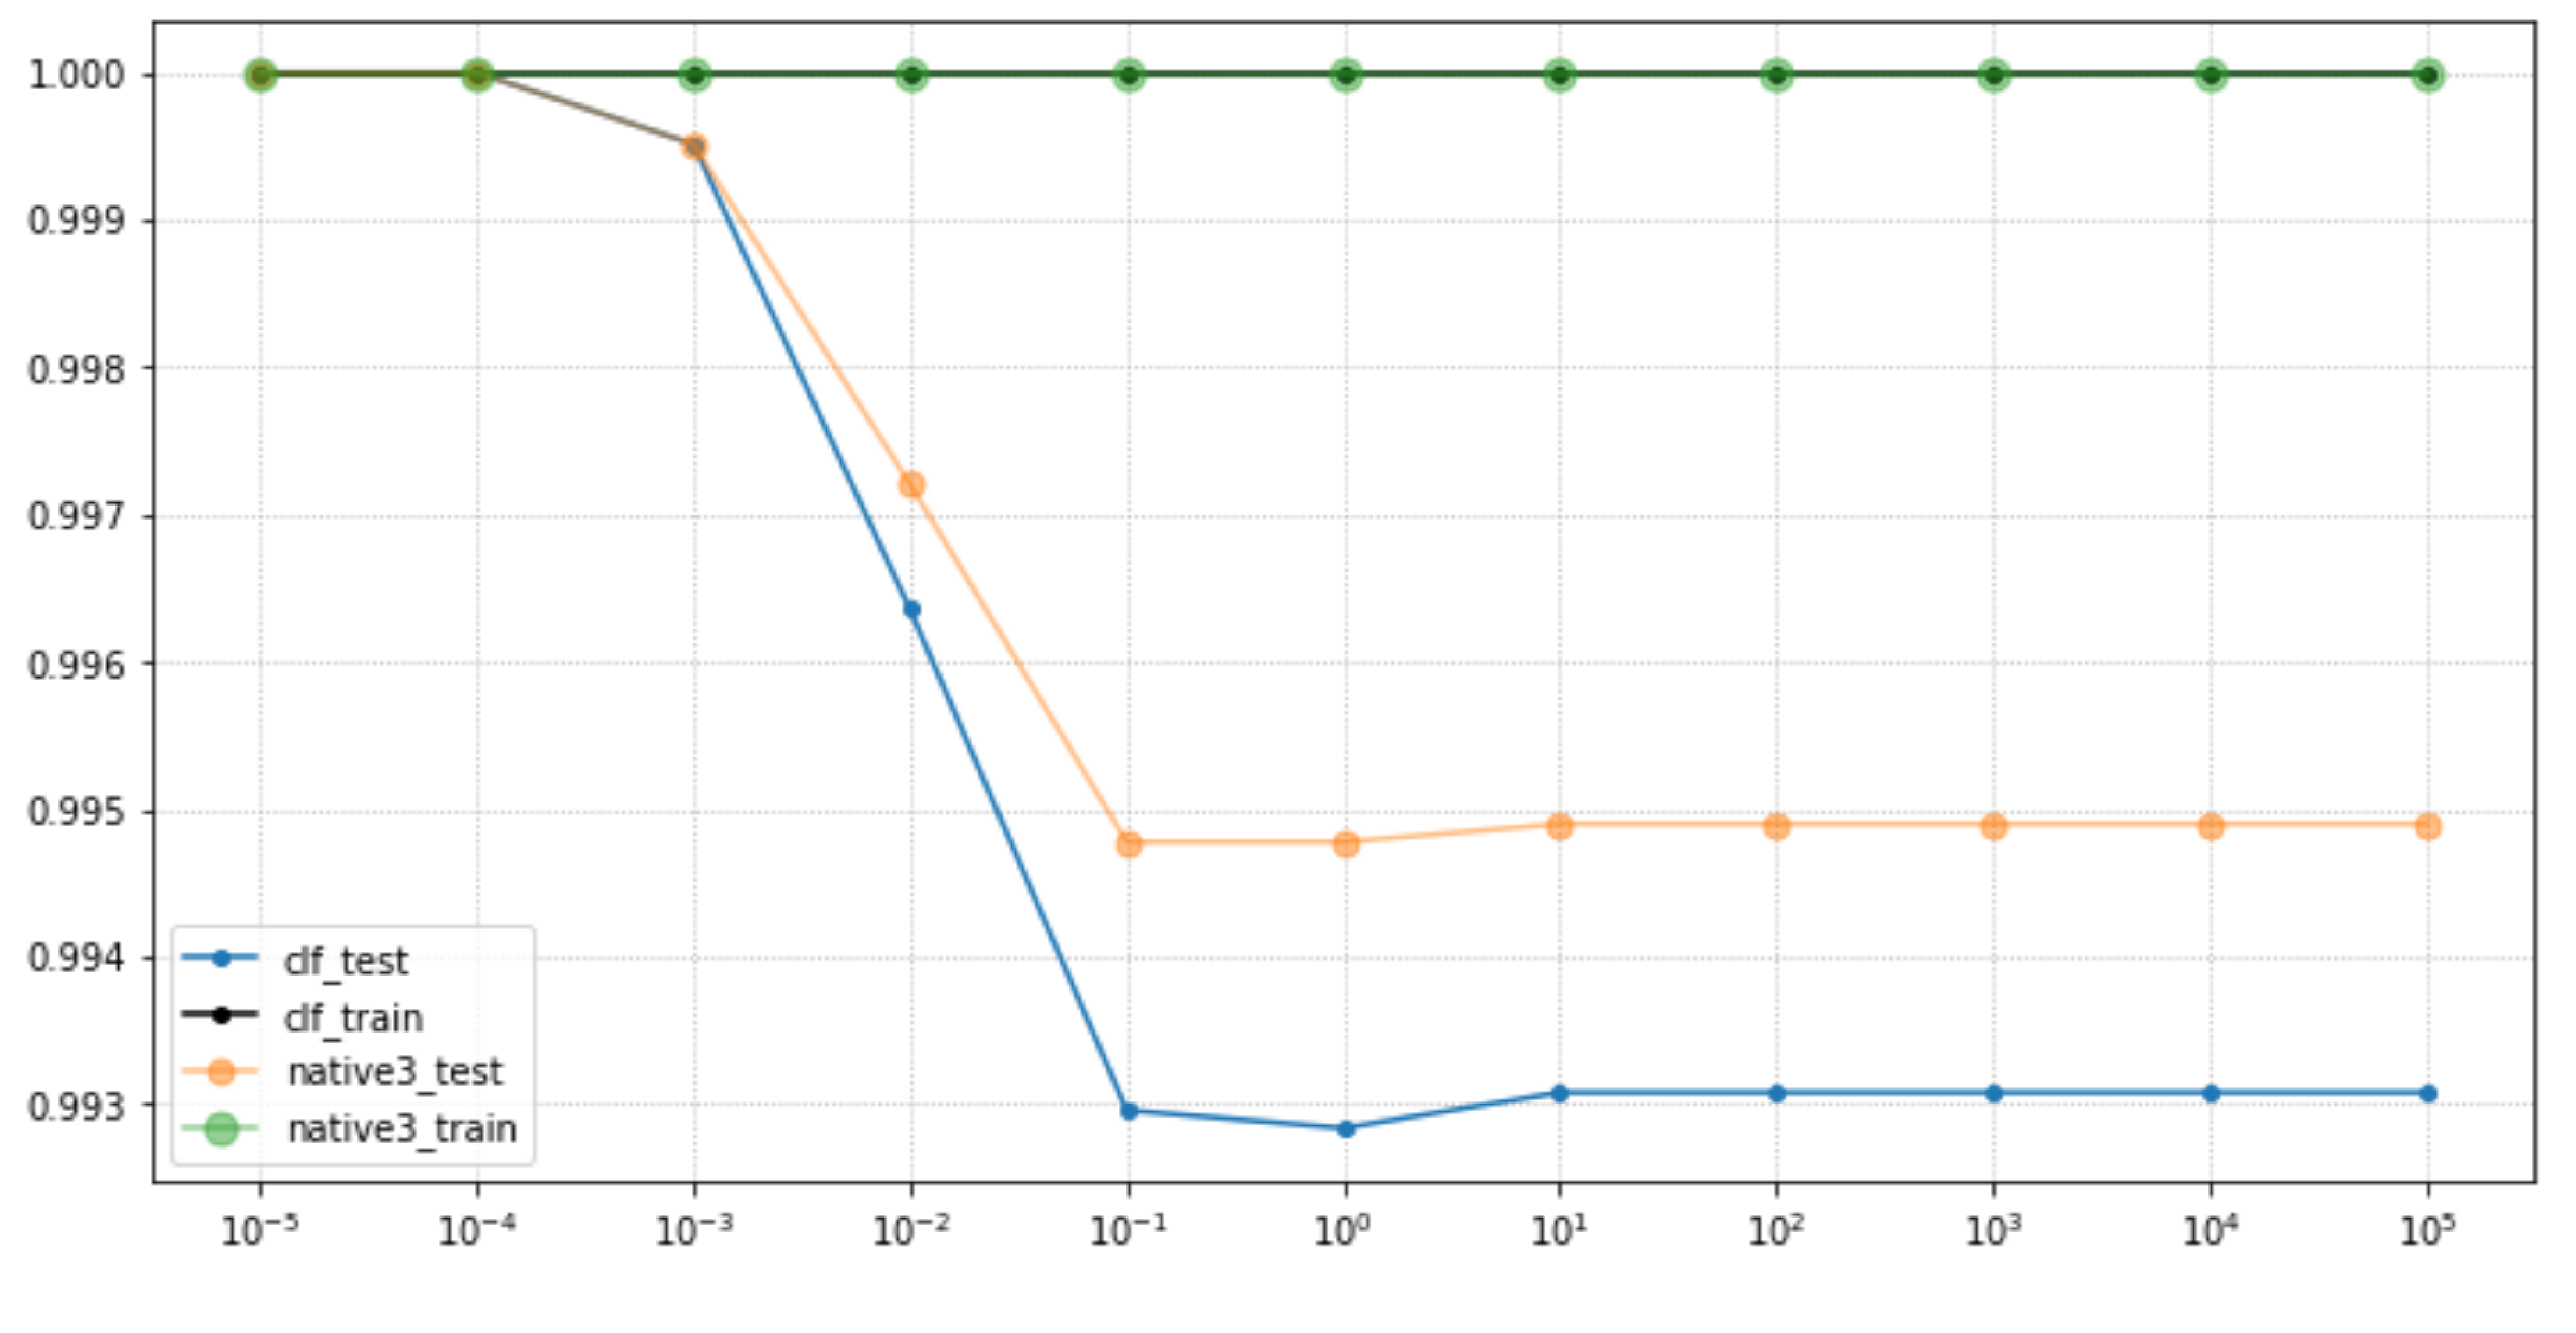
\includegraphics[width=0.5\textwidth]{CLF.eps}}
	\subfloat[MSE]{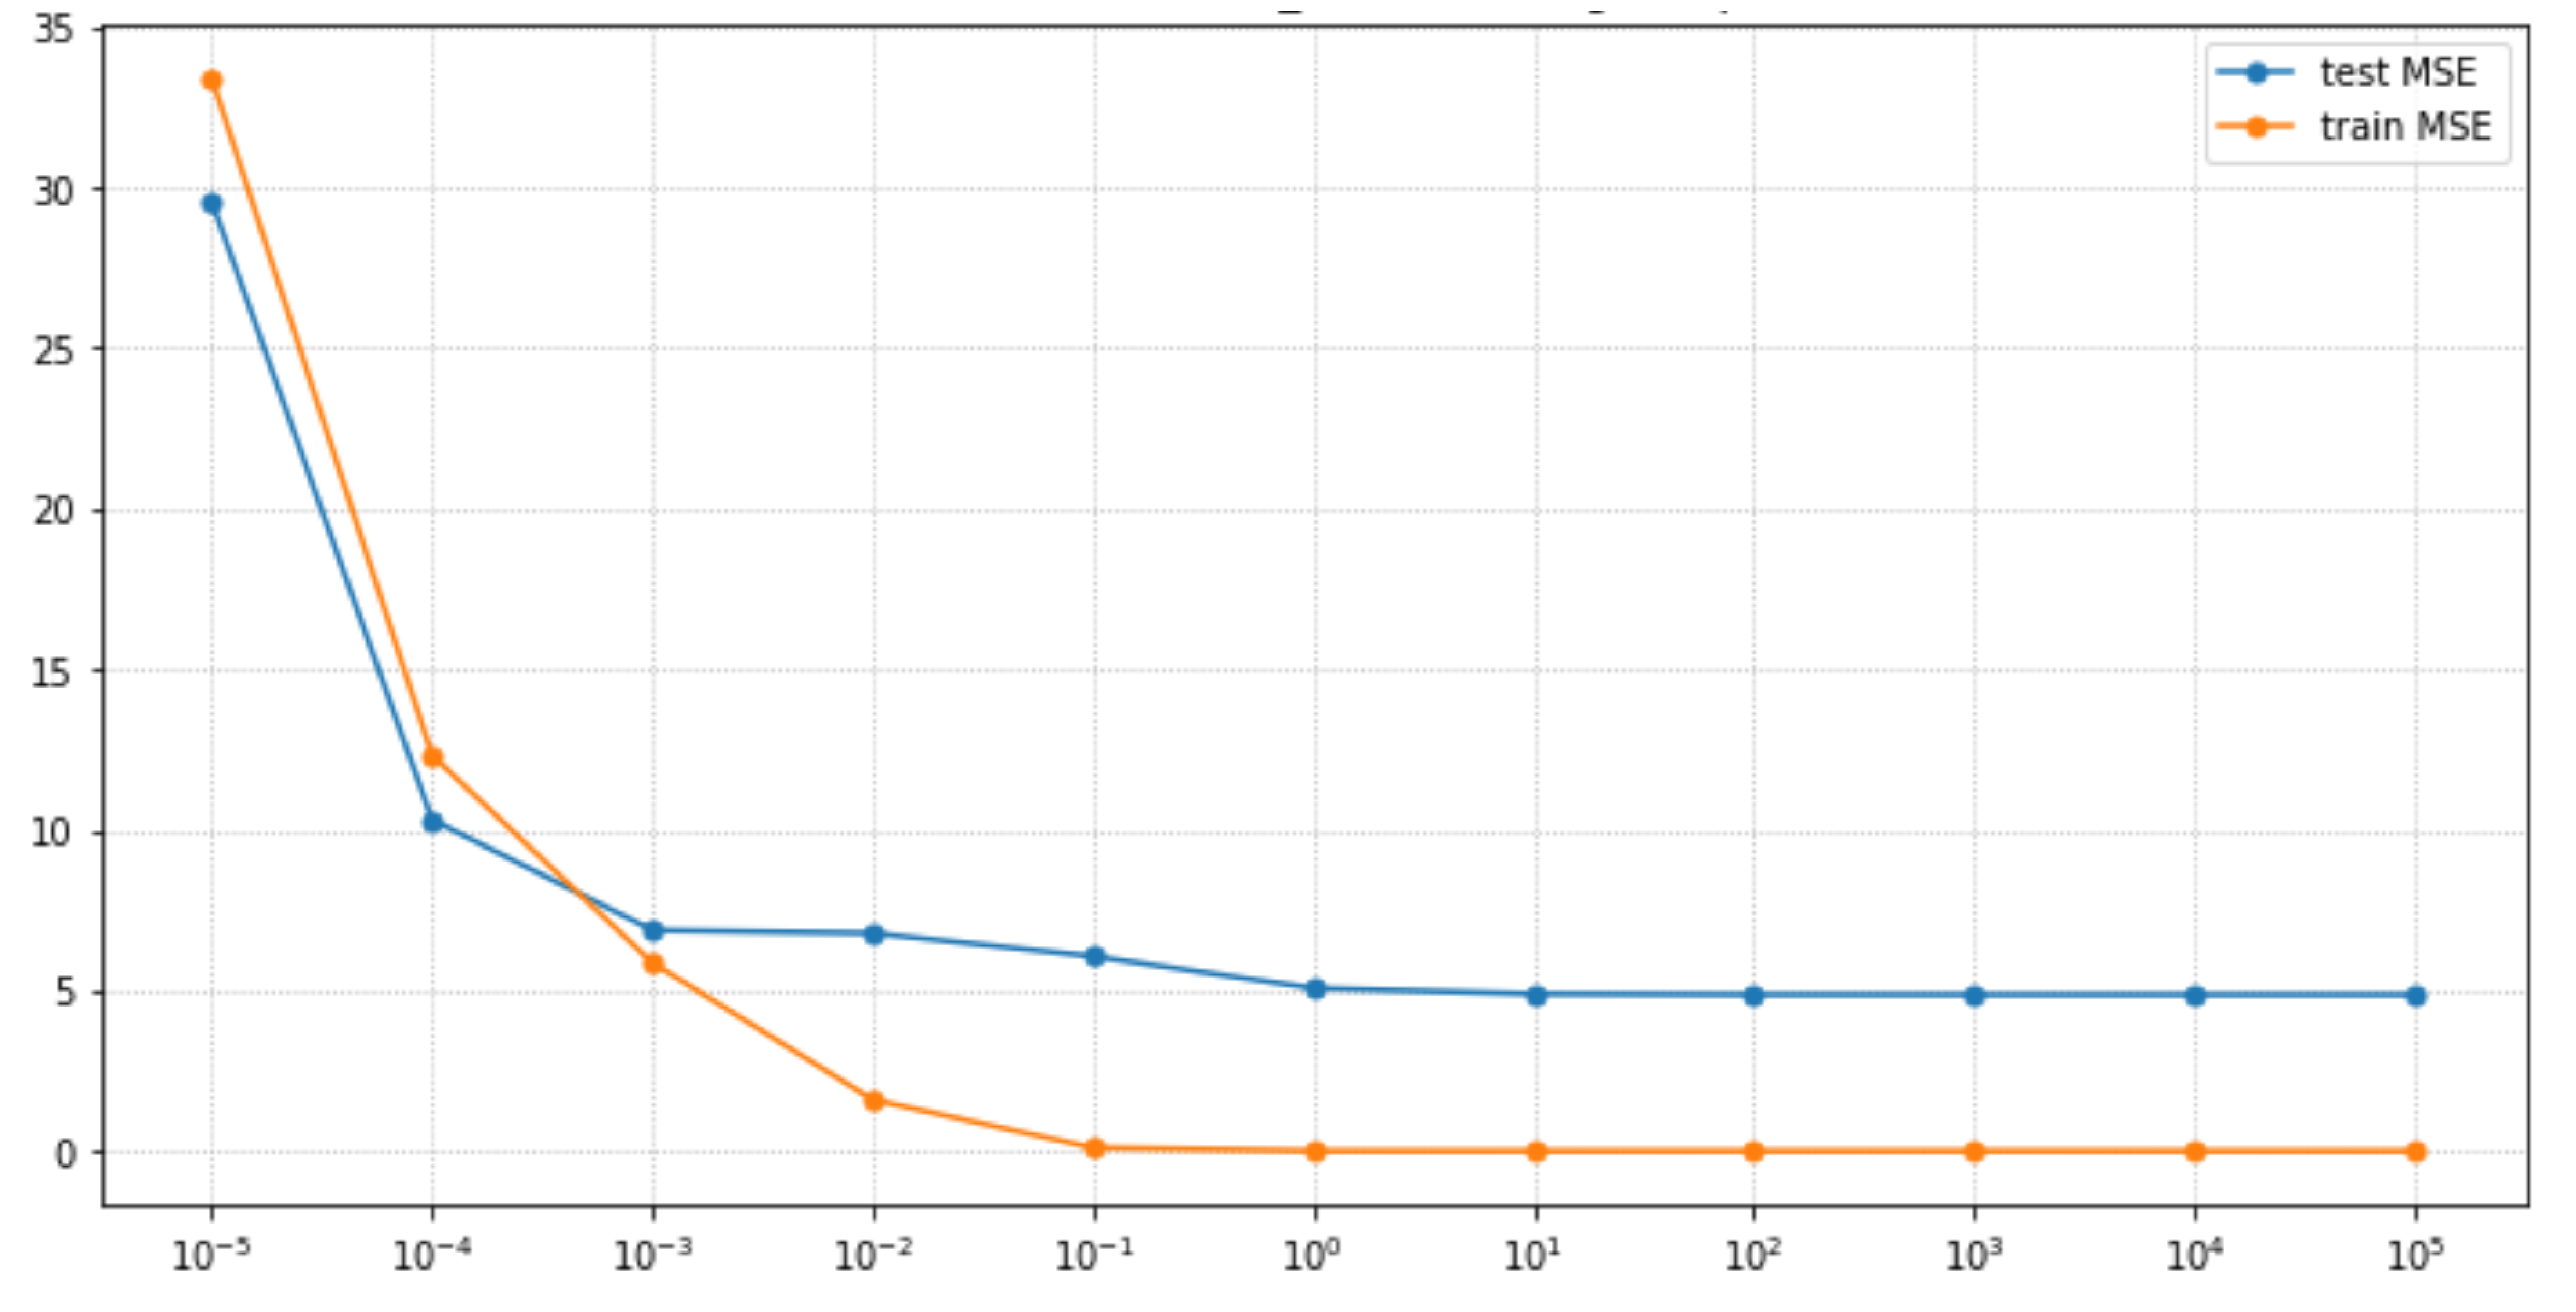
\includegraphics[width=0.5\textwidth]{MSE.eps}}\\
	\label{fg:Example}
\end{figure}

\section{Заключение}


\begin{thebibliography}{1}
	\bibitem{docking} 
	Lengauer T, Rarey M (Jun 1996).  
	\textbf{"Computational methods for biomolecular docking". Current Opinion in Structural Biology}. 
	6 (3): 402–6.
	
	\bibitem{classification} 
	Maria Kadukova, Sergei Grudinin.
	\textbf{Convex-PL: a novel knowledge-based potential for protein-ligand interactions deduced from structural databases using convex optimization}.
	Journal of Computer-Aided Molecular Design, October 2017, Volume 31, Issue 10, pp 943–958.
	
	\bibitem{scoring_functions} 
	Xuan-Yu Meng, Hong-Xing Zhang, Mihaly Mezei, and Meng Cui.
	\textbf{Molecular Docking: A powerful approach for structure-based drug discovery}.
	Curr Comput Aided Drug Des. 2011 Jun 1; 7(2): 146–157.
	
	\bibitem{convex_optimization} 
	S.P. Boyd and L. Vandenberghe.
	\textbf{Convex optimization}.
	Cambridge Univ Press, 2004.
	
	\bibitem{vapnik} 
	V. Vapnik.
	\textbf{The nature of statistical learning theory}.
	Springer, 2000.
	
	\bibitem{D3R}
	Maria Kadukova and Sergei Grudinin.
	\textbf{Docking of small molecules to farnesoid X receptors using AutoDock Vina with the Convex-PL potential : lessons learned from D3R Grand Challenge 2}.
	J. Comput.-Aided Mol. Des., 2017. 
	
	\bibitem{regression} 
	Sergei Grudinin, Maria Kadukova, Andreas Eisenbarth, Simon Marillet, Frédéric Cazals.
	\textbf{Predicting binding poses and affinities for protein-ligand complexes in the 2015 D3R Grand Challenge using a physical model with a statistical parameter estimation}.
	J Comput Aided Mol Des. 2016 Sep;30(9):791-804. Epub 2016 Oct 7.
	
	\bibitem{KRR1} 
	D. Barber.
	\textbf{Bayesian reasoning and machine learning}.
	Cambridge University Press, Cambridge, 2012.
	
	\bibitem{KRR2} 
	Kevin Vu, John Snyder, Li Li, Matthias Rupp, Brandon F. Chen, Tarek Khelif, Klaus-Robert Müller, Kieron Burke.
	\textbf{Understanding Kernel Ridge Regression: Common behaviors from simple functions to density functionals}.
	
	\bibitem{KRR3} 
	Press, WH; Teukolsky, SA; Vetterling, WT; Flannery, BP (2007).
	\textbf{"Section 19.5. Linear Regularization Methods". Numerical Recipes: The Art of Scientific Computing (3rd ed.)}.
	New York: Cambridge University Press. ISBN 978-0-521-88068-8.
	
	\bibitem{rmax1} 
	Sheng-You Huang and Xiaoqin Zou.
	\textbf{An iterative knowledge-based scoring function for protein–protein recognition}.
	Proteins: Struct., Funct., Bioinf., 72(2):557–579, 2008.
	
	\bibitem{rmax2} 
	Gwo-Yu Chuang, Dima Kozakov, Ryan Brenke, Stephen R Comeau, and Sandor Vajda.
	\textbf{Dars (decoys as the reference state) potentials for protein-protein docking}.
	Biophys. J., 95(9):4217–4227, 2008.
	
	\bibitem{rmax3} 
	Vladimir N Maiorov and Gordon M Grippen.
	\textbf{Contact potential that recognizes the correct folding of globular proteins}.
	J. Mol. Biol., 227(3):876–888, 1992.
	
	\bibitem{rmax4} 
	Jian Qiu and Ron Elber.
	\textbf{Atomically detailed potentials to recognize native and approximate protein structures}.
	Proteins: Struct., Funct., Bioinf., 61(1):44–55, 2005.
	
	\bibitem{rmax5} 
	Dror Tobi and Ivet Bahar.
	\textbf{Optimal design of protein docking potentials: Efficiency and limitations}.
	Proteins: Struct., Funct., Bioinf., 62(4):970–981, 2006.
	
	\bibitem{rmax6} 
	Myong-Ho Chae, Florian Krull, Stephan Lorenzen, and Ernst-Walter Knapp.
	\textbf{Predicting protein complex geometries with a neural network}.
	Proteins: Struct., Funct., Bioinf., 78(4):1026–1039, 2010.
	

	
\end{thebibliography}

\end{document}
